% Copyright (c) 2010 Jérémie DECOCK (http://www.jdhp.org)

\documentclass[pdftex,a4paper,11pt]{article} 
\usepackage[utf8]{inputenc}
\usepackage[frenchb]{babel}
\usepackage[pdftex]{graphicx}
\usepackage{amsmath}
\usepackage{subfigure}
\usepackage{hyperref}

\hypersetup{
	pdftoolbar=true,                                          % show Acrobat’s toolbar ?
	pdfmenubar=true,                                          % show Acrobat’s menu ?
	pdffitwindow=true,                                        % page fit to window when opened
	pdftitle={Pyarm}, % title
	pdfauthor={Jérémie DECOCK},                               % author
	pdfsubject={Pyarm}, % subject of the document
	pdfnewwindow=true,                                        % links in new window
	pdfkeywords={Pyarm},           % list of keywords
	colorlinks=true,                                          % false: boxed links; true: colored links
	linkcolor=black,                                          % color of internal links
	citecolor=black,                                          % color of links to bibliography
	filecolor=black,                                          % color of file links
	urlcolor=black                                            % color of external links
}

\begin{document}

\title{Pyarm}
\author{
	Jérémie \bsc{Decock}
}
\date{\today{}}

\maketitle

%%%%%%%%%%%%%%%%%%%%%%%%%%%%%%%%%%%%%%%%%%%%%%%%%%%%%%%%%%%%%%%%%%%%%%%%%%%%%%%%

\section{Présentation des modèles}

\subsection{Présentation}

\begin{center}
        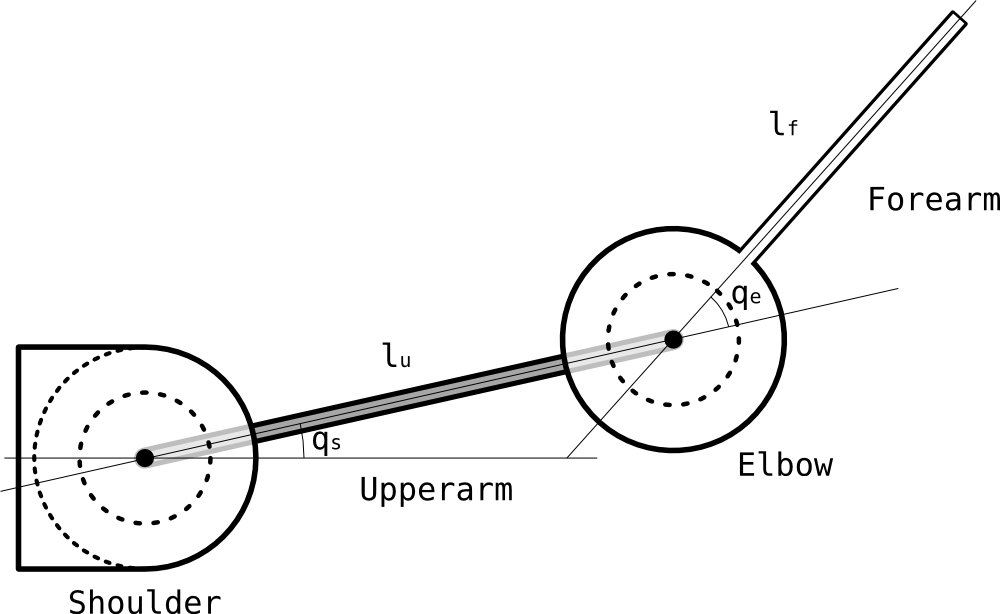
\includegraphics[width=.40\linewidth]{fig/arm}
\end{center}

\begin{itemize}
    \item Bras 2D
    \item Plan horizontal ou vertical
    \item 2 articulations (épaule et coude)
    \item 6 muscles
\end{itemize}

\subsection{Les modèles étudiés}
Trois modèles ont été étudiés :
\begin{itemize}
    \item Katayama / Mitrovic % plan horizontal, refs.
    \item Kambara % plan vertical, refs.
    \item Brown / Weiwei % plan horizontal, refs.
\end{itemize}

\subsection{Simulateur Pyarm}

\begin{itemize}
    \item Codé en Python
    \item Implémente les 3 modèles
\end{itemize}

\begin{figure}
    \centering
    \subfigure{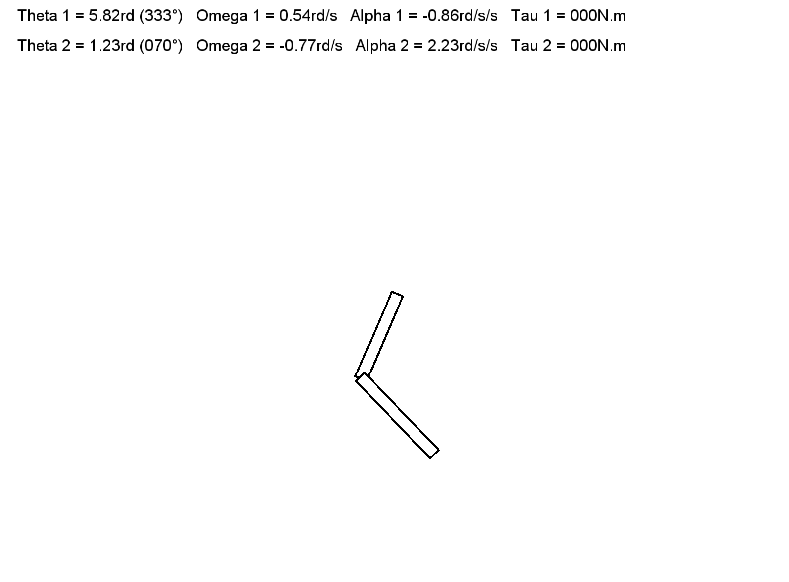
\includegraphics[width=.30\linewidth]{fig/pyarm1}}~~~
    \subfigure{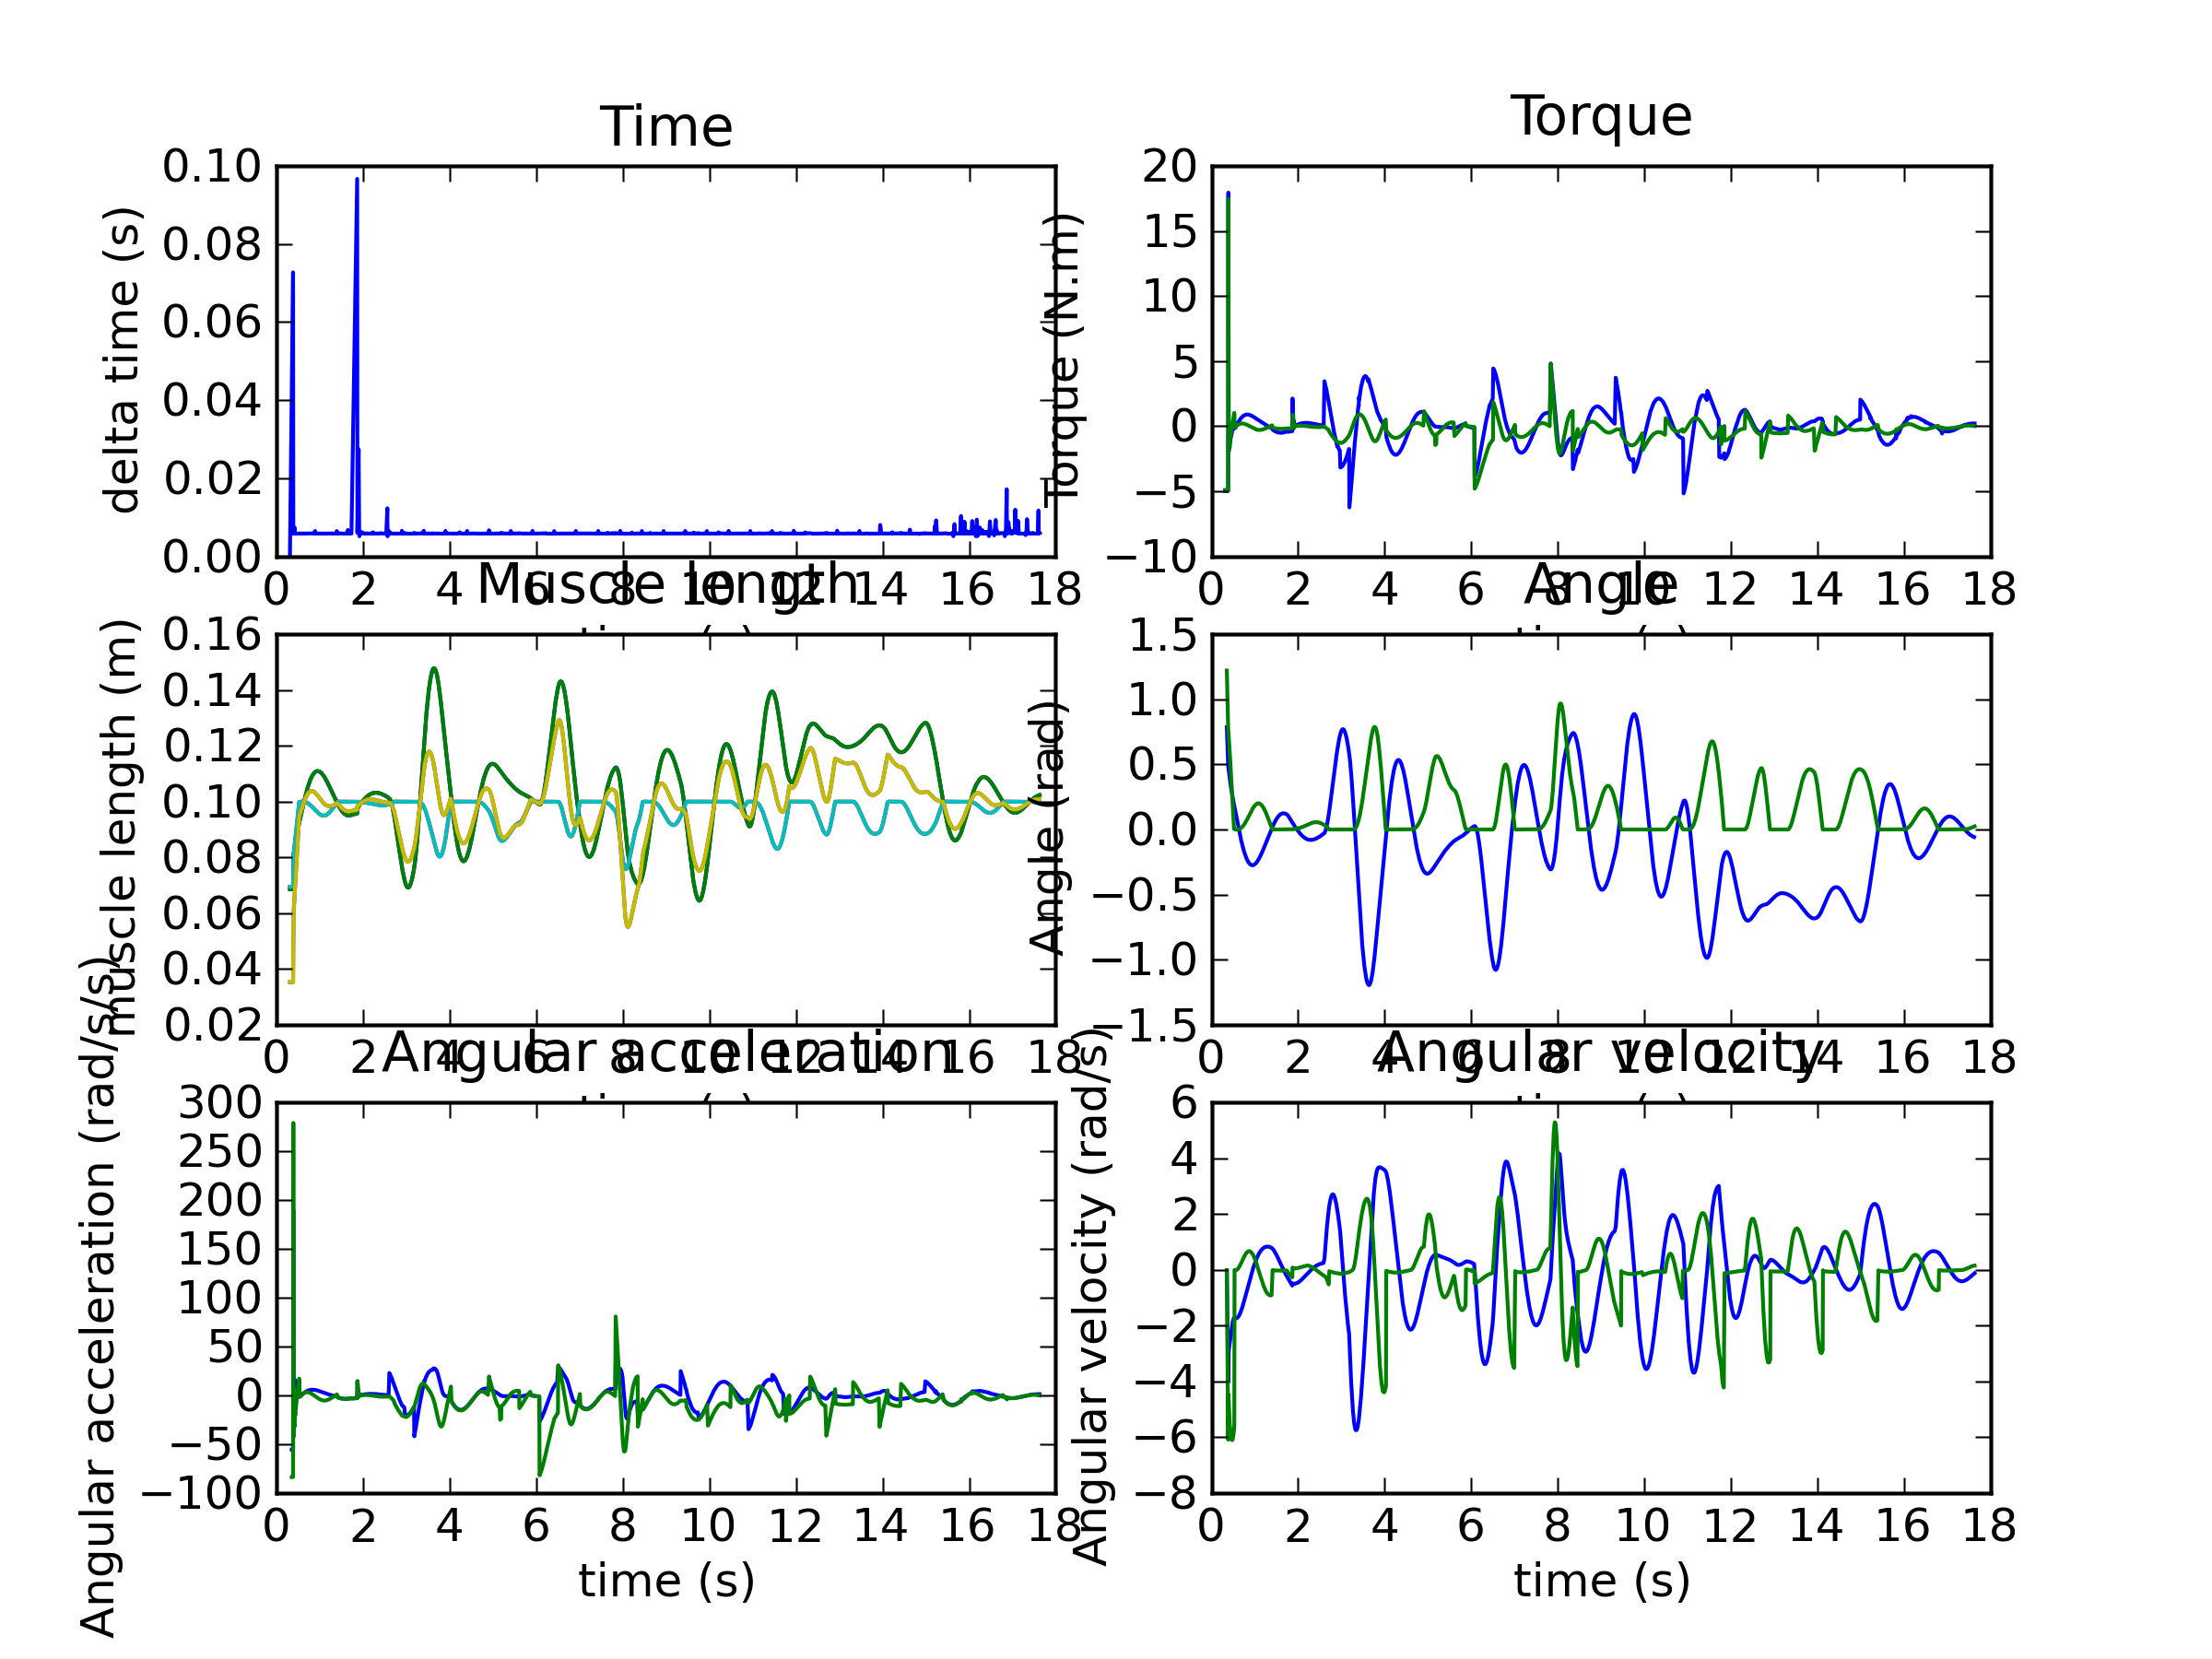
\includegraphics[width=.30\linewidth]{fig/pyarm2}}~~~
    \subfigure{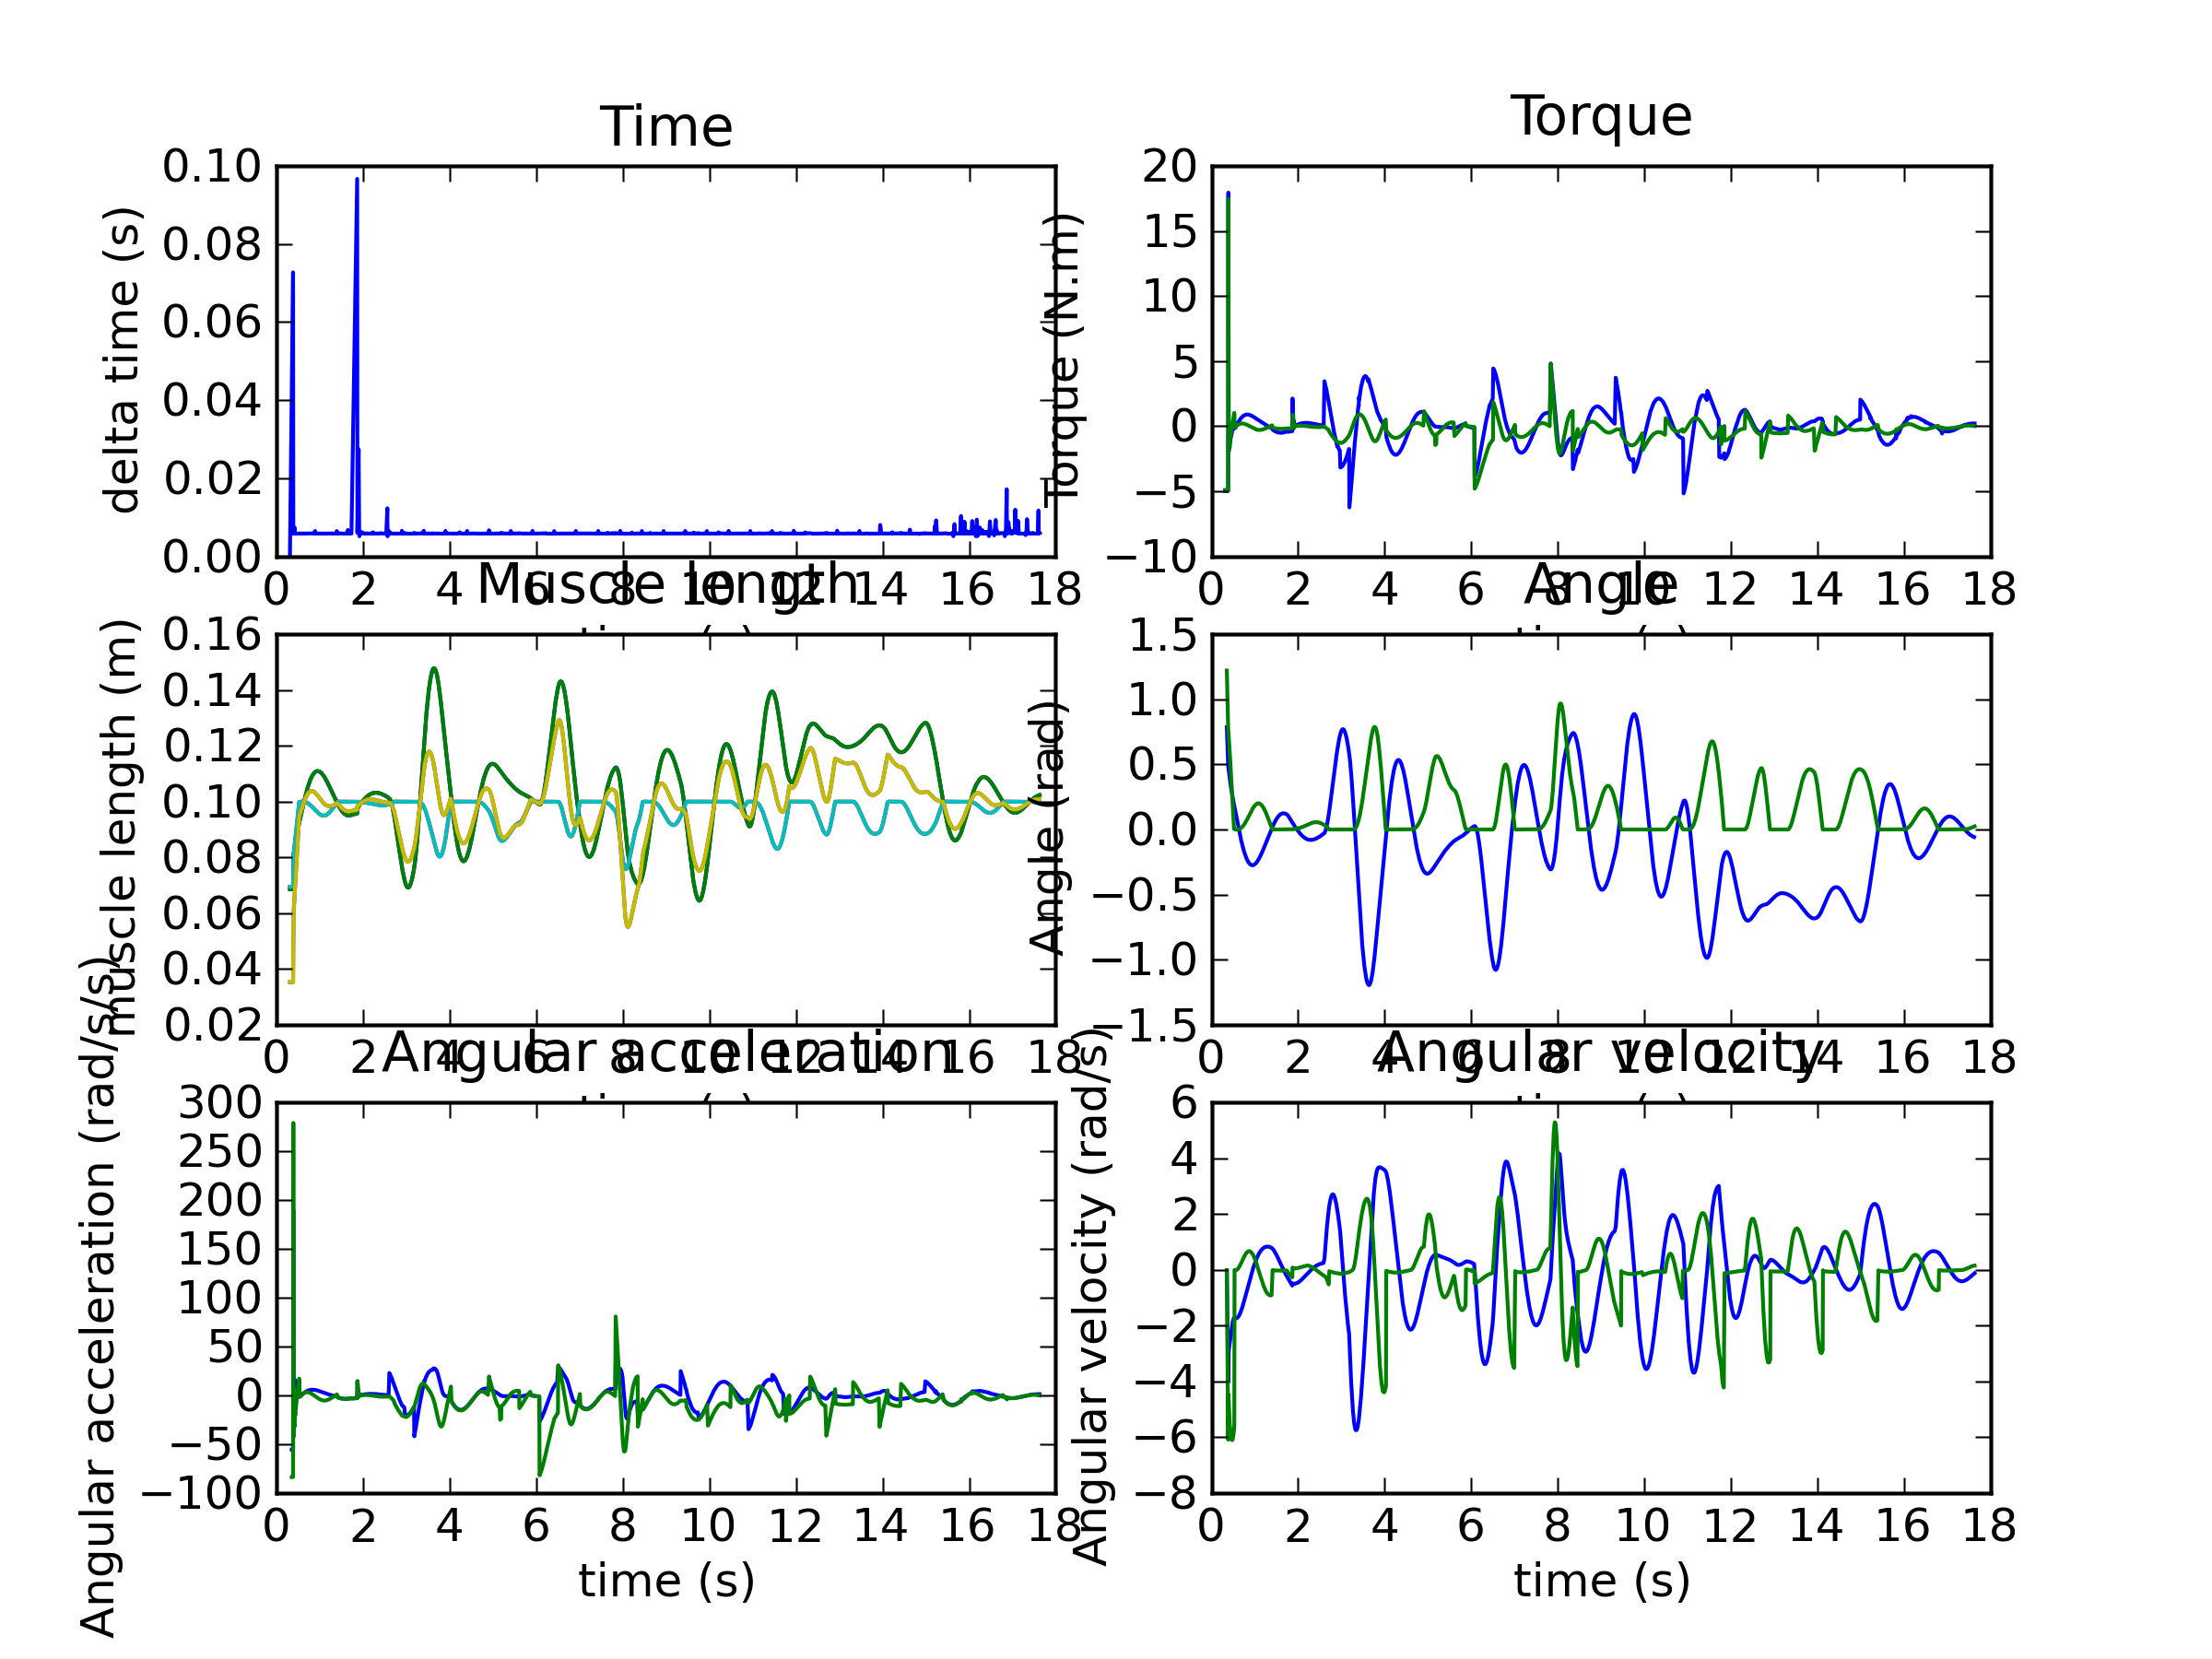
\includegraphics[width=.30\linewidth]{fig/pyarm2}}~~~
\end{figure}

\paragraph{}
Le simulateur est composé de 5 modules :
\begin{itemize}
    \item Filtre sur signal d'entrée
    \item Modèle de bras
    \begin{itemize}
        \item Cinématique
        \item Dynamique
    \end{itemize}
    \item Modèle de muscles
    \begin{itemize}
        \item Cinématique
        \item Dynamique
    \end{itemize}
\end{itemize}

\paragraph{}
TODO (Schéma des modules avec les variables échangées) % TODO

%%%%%%%%%%%%%%%%%%%%%%%%%%%%%%%%%%%%%%%%%%%%%%%%%%%%%%%%%%%%%%%%%%%%%%%%%%%%%%%%

\section{Modèle de bras}

%%%%%%%%

\subsection{Cas général}

\subsubsection{Dynamique inverse}
$\tau = M(\theta)\alpha + C(\theta, \omega) + b(\omega) + g(\theta) $

\subsubsection{Dynamique}
$\alpha = M(\theta)^{-1} + (\tau - C(\theta, \omega) - b(\omega) - g(\theta)) $

\subsubsection{Légende}
\begin{tabular}{lcl}
    $M$      & = & matrice des moments d'inertie \\ % TODO
    $C$      & = & force de Coriolis et force centripète \\
    $b$      & = & force de viscosité et de friction \\ % TODO
    $g$      & = & force de gravité \\
    $\tau$   & = & couple total exercé sur les articulations ($N.m$) \\
    $\alpha$ & = & accélération angulaire ($rd.s^{-2}$) \\
    $\omega$ & = & vitesse angulaire ($rd.s^{-1}$) \\
    $\theta$ & = & angle ($rd$) \\
\end{tabular}

%%%%%%%%

\subsection{Mitrovic}

\subsubsection{Dynamique inverse}
$\tau = M(\theta)\alpha + C(\theta, \omega) \omega $

\subsubsection{Dynamique}
$\alpha = M(\theta)^{-1} + (\tau - C(\theta, \omega) \omega) $

%%%%%%%%

\subsection{Kambara}

\subsubsection{Dynamique inverse}
$
\begin{pmatrix}
    \tau_1 \\
    \tau_2 \\
\end{pmatrix}
=
\begin{pmatrix}
    M_{11}\alpha_1 + M_{12}\alpha_2 + h_{122}\omega_2^2 + 2h_{112}\omega_1\omega_2 + g_1 \\
    M_{21}\alpha_1 + M_{22}\alpha_2 + h_{211}\omega_1^2 + g_2 \\
\end{pmatrix}
(1)$

\paragraph{}
\begin{tabular}{lcl}
    $M_{11}$ & = & $I_1 + I_2 + m_2(l_1^2 + 2 l_1 l_{g2}\cos\theta_2$) \\
    $M_{12}$ & = & $I_2 + m_2l_1l_{g2}\cos\theta_2$ \\
    $M_{21}$ & = & $I_2 + m_2l_1l_{g2}\cos\theta_2$ \\
    $M_{22}$ & = & $I_2$ \\
    $h_{122}$ & = & $-m_2 l_1 l_{g2} \sin\theta_2$ \\
    $h_{112}$ & = & $-m_2 l_1 l_{g2} \sin\theta_2$ \\
    $h_{211}$ & = & $m_2 l_1 l_{g2} \sin\theta_2$ \\
    $g_1$ & = & $m_1 g l_{g1} \cos\theta_1 + m_2 g(l_1 \cos\theta_1 + l_{g2} \cos(\theta_1 + \theta_2))$ \\
    $g_2$ & = & $m_2 g l_{g2} \cos(\theta_1 + \theta_2))$ \\
    & & \\
    $m_j$ & = & masse du membre \\
    $l_j$ & = & longueur du membre \\
    $l_{gj}$ & = & distance séparant le centre de masse de l'articulation \\
    $I_{j}$ & = & moment d'inertie \\
\end{tabular}

\paragraph{}
\begin{tabular}{lcl}
    (1) & $\Leftrightarrow$ & $\tau = M(\theta)\alpha + C(\theta, \omega) \omega + g$ \\
\end{tabular}

\subsubsection{Dynamique}
$\alpha = M(\theta)^{-1} + (\tau - C(\theta, \omega) \omega - g) $

%%%%%%%%

\subsection{Weiwei}

\subsubsection{Dynamique inverse}
$\tau = M(\theta)\alpha + C(\theta, \omega) + B\omega $

\paragraph{}
\begin{tabular}{lcl}
    $M$ & = &
    $
    \begin{pmatrix}
        d1 + 2 d_2 \cos\theta_2  & d_3 + d_2 \cos \theta_2 \\
        d_3 + d_2 \cos\theta_2 & d_3 \\
    \end{pmatrix}
    $ \\

    $C$ & = &
    $
    \begin{pmatrix}
        -\omega_2 (2 \omega_1 + \omega_2) \\
        \omega_1^2 \\
    \end{pmatrix}
    d_2 \sin\theta_2
    $\\

    $B$ & = &
    $
    \begin{pmatrix}
        0.05  & 0.025 \\
        0.025 & 0.05 \\
    \end{pmatrix}
    $
\end{tabular}

\paragraph{}
\begin{tabular}{lcl}
    $d_1$ & = & $I_1 + I_2 + m_2 l_1^2$ \\
    $d_2$ & = & $m_2 l_1 s_2$ \\
    $d_3$ & = & $I_2$ \\
\end{tabular}

\paragraph{}
\begin{tabular}{lcl}
    $m_j$ & = & masse du membre \\
    $l_j$ & = & longueur du membre \\
    $s_{j}$ & = & distance séparant le centre de masse de l'articulation \\
    $I_{j}$ & = & moment d'inertie \\
\end{tabular}

\subsubsection{Dynamique}
$\alpha = M(\theta)^{-1} + (\tau - C(\theta, \omega) - B\omega) $


%%%%%%%%%%%%%%%%%%%%%%%%%%%%%%%%%%%%%%%%%%%%%%%%%%%%%%%%%%%%%%%%%%%%%%%%%%%%%%%%

\section{Modèle de muscles}

\subsection{Mitrovic}

\subsection{Kambara}

\subsection{Weiwei}

\begin{center}
        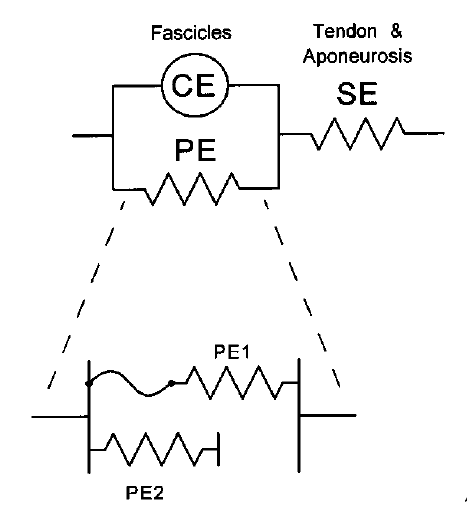
\includegraphics[width=.40\linewidth]{fig/brown}
\end{center}

\begin{tabular}{lcl}
    $CE$  & = & éléments contractiles \\
    $SE$  & = & élasticité des tendons (ignorée) \\
    $PE$  & = & élasticité du muscle \\
    $PE1$ & = & résistance à l'étirement du muscle passif \\
    $PE2$ & = & résistance à la compression du muscle actif \\
\end{tabular}


%%%%%%%%%%%%%%%%%%%%%%%%%%%%%%%%%%%%%%%%%%%%%%%%%%%%%%%%%%%%%%%%%%%%%%%%%%%%%%%%

\end{document}
